\documentclass[11pt,journal,compsoc]{IEEEtran}
\usepackage[colorlinks,linkcolor=blue]{hyperref}
\usepackage{indentfirst}
\usepackage{graphicx}
\usepackage{caption}
\usepackage{subfigure}
\setlength{\parindent}{2em}
\ifCLASSOPTIONcompsoc
  \usepackage[nocompress]{cite}
\else
  \usepackage{cite}
\fi
\renewcommand{\thesubfigure}{\thefigure.\arabic{subfigure}} 
\makeatletter 
\renewcommand{\@thesubfigure}{\thesubfigure:\space} \renewcommand{\p@subfigure}{}
\makeatother

\hyphenation{op-tical net-works semi-conduc-tor}

\begin{document}
\title{3D ShapeNets: A Deep Representation for Volumetric Shape Modeling}
\author{Yangling Zhang, Wanxin Qu}

\markboth{CS337 -- Computer Graphics --- Group P2}
{Shell \MakeLowercase{\textit{et al.}}: Bare Demo of IEEEtran.cls for Computer Society Journals}

\IEEEtitleabstractindextext{
  \begin{abstract}
    The paper \textit{3D ShapeNets: A Deep Representation for Volumetric Shape Modeling} introduces a new representation of 3D objects and build a model 3D ShapeNets, which learns the distribution of complex 3D shapes for different object classes and arbitrary poses. And it can perform joint object recognition and shape reconstruction from 2.5D depth maps and active object recognition through view planning. We change the parameters of the model, improve the accuracy of the recognition. Based on this, we build a new model with a different architecture for object recognition. The test result shows the new model works well. 
    
    % and implements a 3D object classification strategy based on CNNs.
  \end{abstract}

  \begin{IEEEkeywords}
    3D ShapeNets,\quad categories\ recognition,\quad architecture,\quad 2.5D\ shape\ nets,\quad CNN, \quad convolutional layers,\quad fully-connected layers, \quad CDBN
  \end{IEEEkeywords}
}

\maketitle

\IEEEdisplaynontitleabstractindextext

\IEEEpeerreviewmaketitle

\IEEEraisesectionheading
  {
  \section{Introduction}\label{sec:introduction}
  }
  \IEEEPARstart{R}{ecognizing} 3D geometric shape has been considered one of the most important cues in object recognition. However, 3D shape is a crucial but heavily underutilized cue in today’s computer vision system, mostly due to the lack of a good generic shape representation. Nowadays with the recent availability of inexpensive 2.5D depth sensors (e.g. MicrosoftKinect), it is becoming increasingly important to have a powerful 3D shape model in the loop.

  In addition to category recognition, another challenging task is to complete the shape from a 2.5D depth map. Recovering these incomplete 3D shapes to full 3D is ciritical for analyzing shape variations. The paper infer the full 3D volume from a 2.5D depth map without the knowledge of the object category.   
  
  The paper proposed 3D ShapeNets to represent a geometric 3D shape. It uses the probabilistic distribution of binary variables on a 3D voxel grid. The model uses a powerful Convolutional Deep Belief Network to learn the complex joint distribution of all 3D voxels in a data driven manner. The model is powerful to recognize objects in single-view 2.5D depth images and calculate the missing parts of depth maps. It also predicts the next-best-view in view planning for active object recognition. 
  
  To represent the probability distribution of these binary variables for 3D shapes, we design a Convolutional Deep Belief Network (CDBN). Deep Belief Networks (DBN) are a powerful class of probabilistic models often used to model the joint probabilistic distribution over pixels and
  labels in 2D images. The paper adapt the model from 2D pixel data to 3D voxel data, which imposes some unique challenges. It propose to use convolution to reduce model parameters by weight sharing. However, different from typical convolutional deep learning models, it has no form of pooling in the hidden layers. Because pooling may enhance the invariance properties for recognition, which would also lead to greater uncertainty for shape reconstruction.
  
  After training the CDBN, the model learns the joint distribution of voxel data and the category label. It is able to recognize objects in single-view 2.5D depth maps. First the 2.5D depth map is converted to a volumetric representation. Then define it as free space, surface or occluded.

  For both human and computer, recognizing objects from a single view is challenging. But one can reduce uncertainty by observing from different side of the object. When given the present view, the model can predict the next best view when recognizing the category. 

  Based on the paper 3D ShapeNets, we modify the model and thus improve the performance in classification. And we test the performance of different angles to find the best angle intervals for training and testing. 
  
  However, the 3D ShapeNets architecture consists of three convolutional layers and two fully connected layers with a large number of parameters, which means that learning requires a large amount of training data sets.

  We build a new model with a different architecture on the basis of the original one to improve the accuracy of 3D object classification. We remove two layers and then expand the width and depth on the remaining three-layer frame.

  Besides, we write a simple testing program in python. Seen from the results, all above perform well.
  
  \hfill January 4, 2019

  \section{Our Work}
  \subsection{Finding the best interval}
  In the paper, the author choose 30 as the degree interval. We want to find whether it is the best interval, regarding to time consumption and the accuracy performance. 

  First we choose$10/30/60/90/180/360^{\circ}$ as the interval to augment the data by rotating each 3D model every certain degrees along the gravity direction. And then test the performance with the testing data of the same angle intervals as the training data. 

  Then we fix the angle interval in test data as 60 degrees, which is the common interval for people to observe an object when they have to change the view side. We test the performance of different models trained with different angle intervals of $10/30/60/90/180/360^{\circ}$. All the results obtained will be explained later in Part 3.

  We also try to increase the amount of training data of the model. Without doubt, the accuracy is improved, but the improvements is not significant. Purely increasing the training data is not economical due to the high time consumption and the low accuracy performance. 
  \subsection{Modify the model}
  Similar to the paper we represent a geometric 3D shape as a probability distribution of binary variables on a 3D voxel grid. Each 3D mesh is represented as a binary tensor: 1 indicates the voxel is inside the mesh surface, and 0 indicates the voxel is outside the mesh. We allocate 2 grid sizes in our experiments which are 30$\times$30$\times$30 and 21$\times$21$\times$21.
  
  In the paper a 3D shape is represented as a 24$\times$24$\times$24 voxel grid with 3 extra cells of padding in both directions to reduce the convolution border artifacts. The first layer has 48 filters of size 6 and stride 2. The second layer has 160 filters of size 5 and stride 2. The third layer has 512 filters of size 4 and stride 1. The fourth layer is a standard fully connected RBM with 1200 hidden units. The fifth and final layer has 4000 hidden units. 
  The architecture of model is the same as the paper provides, which is shown in Fig1.1a.

  For our 21$\times$21$\times$21 grid size, a 3D shape is represented as a 21$\times$21$\times$21 voxel grid with no extra cells of padding. The first layer has 48 filters of size 7 and stride 1. The second layer has 160 filters of size 5 and stride 2. The third layer has 512 filters of size 4 and stride 1. The fourth layer is a standard fully connected RBM with 1200 hidden units. The fifth and final layer has 4000 hidden units.The architecture is as Fig1.2b shows.

  \begin{figure}[htbp]
    \centering
    \subfigure[a]{
      \begin{minipage}{4cm}
      \centering
      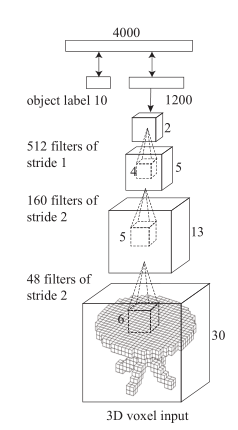
\includegraphics[width=4cm]{pic/arch1.png}
      \end{minipage}}
    \subfigure[b]{
      \begin{minipage}{4cm}
      \centering
      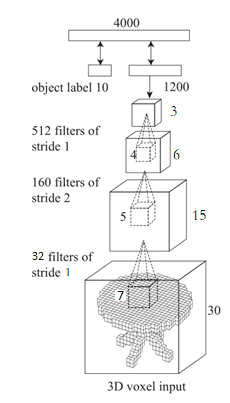
\includegraphics[width=4cm]{pic/arch2.png}
      \end{minipage}}
    \caption{Model Architecture of Different Parameters}
  \end{figure}

  \subsection{A New Architecture}
  The work above is all the parameter changes on the original architecture. Next is the change to the model architecture.

  In 3D ShapeNets, the architecture contains 3 convolutional layers and 2 fully-connected layers, with total 12M parameters. This means the model needs large training datasets. But comparing with common datasets used in other domains, present available 3D shape datasets are smaller by at least an magnitude. Thus we conducts a model pursuit for robust learning of 3D CNN, with 150 times fewer parameters than 3D ShapeNets.
  
  We try different combinations of convolutional layers and fully-connected layers, and finally get the optimal architecture.The model contains only three convolutional layers and one fully connected layers. The first convolutional layers has 16 filters of size 6 and stride 2. The second onvolutional layers has 64 filter of size 5 and stride 2. The third convolutional layers has 64 filter of size 5 and stride 2. The fully connected layer has 400 hidden units. 
  \begin{figure}[ht]
    \centering
    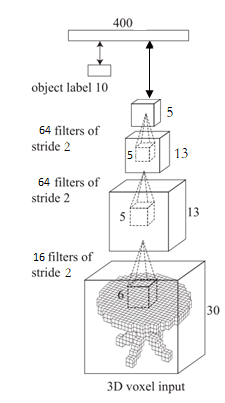
\includegraphics[width=4cm]{pic/arch3.png}
    \caption{New Model}
    \label{figure:label}
  \end{figure}
  \subsection{A Simple Test}
  We provide 4 functions in file utils.py, three of which just for load. The rest one prints and plots the confusion matrix.

  \section{Result}
  In Part 3.1 and 3.2, we process the data of ModelNet40 for training. In Part 3.3 we use both ModelNet40 and ModelNet10.

  \subsection{Testing On The Previous Model}
  In this part we train models according to the paper with only the training data and test data changed.We tested them and get some conclusions. The first change is the angle and test data set. We obtain correspondences between accuracy and angle in two cases. 
  When the training data set tests the corresponding model, the correspondence is as Table1 and Fig3 show. 180 is the best interval for training and test theoretically. This can be explained that the more angles of view the model have to learn the worse it learns. This is like  comparing taking 1 class in a semester with taking 10 classes in the same semester for the same student. Which is for sure, the less class the student have to learn, the better the student learns. In addition, when when the number of the training data is limited due to the time limits, the larger angle interval can cover more situation of viewing which in a word indicates more diversity. However, if we choose 360 as the angle interval, there are not enough data for training, thus cause the performance not as pleasant as 180.

  \begin{table}[ht]
  \caption{angle-accuracy table(dateset tests corresponding model} % title of Table
  \centering % used for centering table
    \begin{tabular}{|c|c|c|c|c|c|c|}
    \hline 
    angle\_inc/$^{\circ}$&10&30&60\\
    \hline  
    accuracy/\%&72.880&82.330&81.000\\
    \hline 
    angle\_inc/$^{\circ}$&90&180&360\\
    \hline  
    accuracy/\%&85.974&86.784&86.903\\
    \hline 
    \end{tabular}
  \end{table}
  
  \begin{figure}[ht]
    \centering
    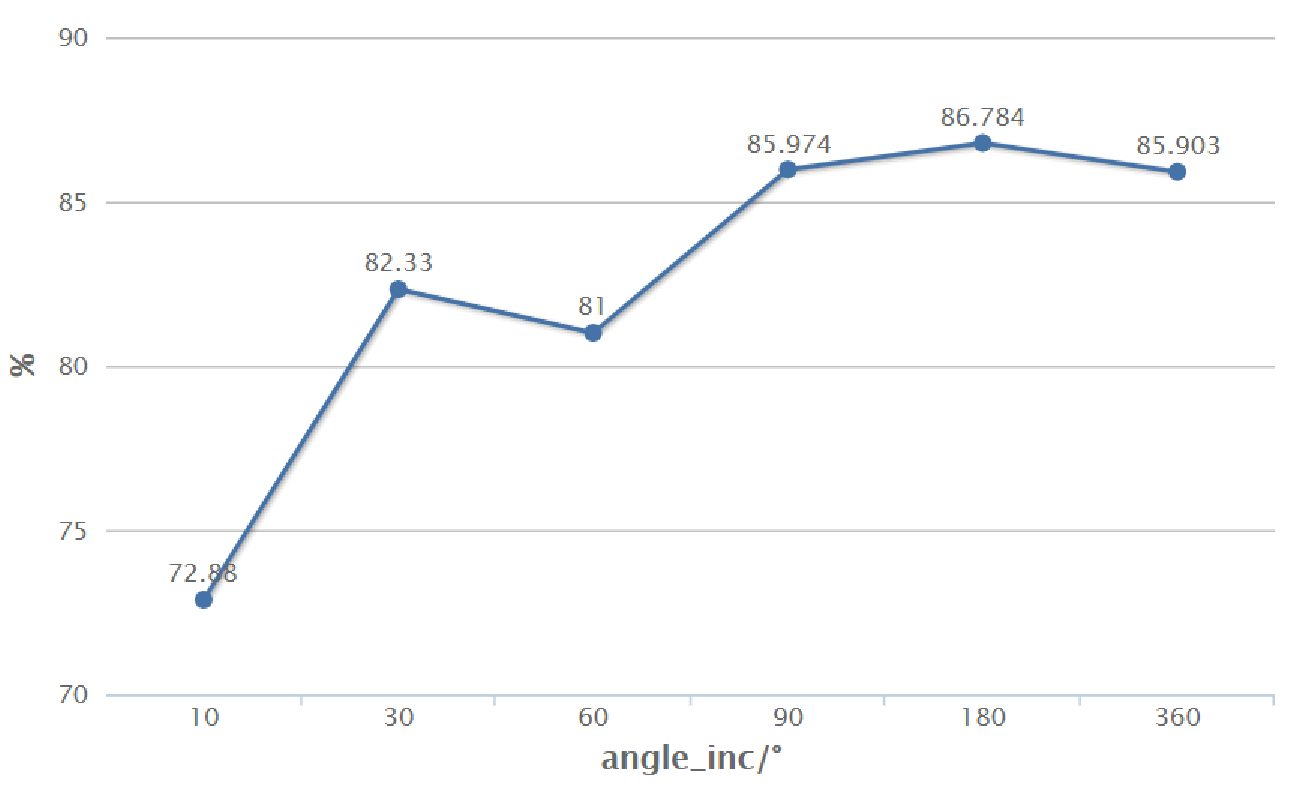
\includegraphics[width=8cm]{pic/result1.png}
    \caption{angle-accuracy chart(dateset tests corresponding model}
    \label{figure:label}
  \end{figure}

  Correspondence between accuracy and angle when the same data set(60$^{\circ}$) tests the corresponding model is as Table2 and Fig4 show. The result shows 30 degree is the best interval. For those large interval trained model, when viewing the object from an angle they have not learned they can not recognize the object correctly. And for those with small intervals, the over-fitting problem can be more critical when the interval goes down. As for the time consumptions are approximately the same, choosing 30 degree as the interval is the best option.
  
  \begin{table}[ht]
    \caption{angle-accuracy table(the same dateset tests all models} % title of Table
    \centering % used for centering table
      \begin{tabular}{|c|c|c|c|c|c|c|}
      \hline 
      angle\_inc/$^{\circ}$&10&30&60\\
      \hline  
      accuracy/\%&76.88&81.63&81.000\\
      \hline 
      angle\_inc/$^{\circ}$&90&180&360\\
      \hline  
      accuracy/\%&72.21&56.27&49.08\\
      \hline 
      \end{tabular}
  \end{table}

  \begin{figure}[ht]
    \centering
    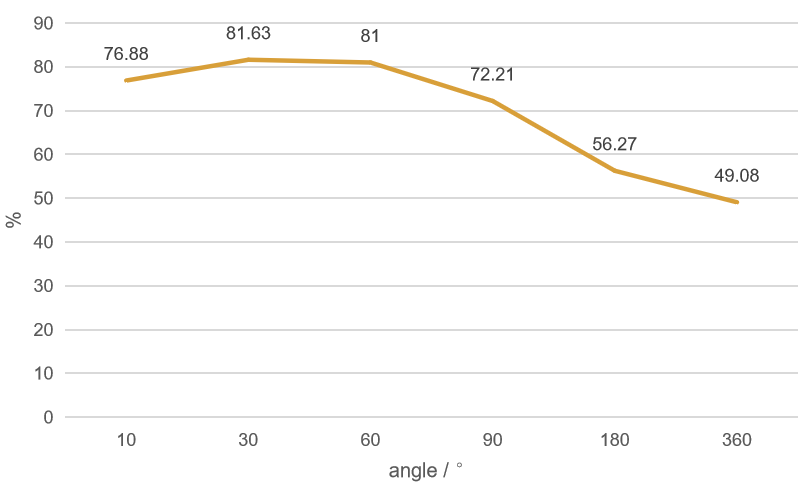
\includegraphics[width=8cm]{pic/result2.png}
    \caption{angle-accuracy chart(the same dateset tests all models}
    \label{figure:label}
  \end{figure}

  Then we increase the amount of training data for the model. There is no doubt that the accuracy is improved.But at the same time, training time is greatly increased. The increased accuracy rate is not proportional to the consuming time. So we can just ignore it.

  \subsection{Model With New Parameters Of The Same Architecture}
  We use 30 degrees to process data at intervals and train the model. Then we test and get an accuracy in classification, which is 87.36\%. Our new model outperform the original one.

  \subsection{New Achitecture}
  Before confirming the final architecture, we try different combinations of convolutional layers and fully-connected layers. And get various results. Here are all combinations we try and the corresponding accuracy.
  (m+n means m conv+n fc, ie.m convolutional layers and n fully-connected layers)

  \begin{table}[ht]
    \caption{Accuracy of different model} % title of Table
    \centering % used for centering table
    \begin{tabular}{|c|c|c|c|c|}
    \hline 
    model(conv+fc)&2+1&2+2&3+1&3+2\\
    \hline  
    train acc/\%&97.719&97.936&94.479&98.583\\
    \hline 
    test acc/\%&78.542&81.958&76.417&80.750\\
    \hline 
    \end{tabular}
  \end{table}
  
  We respectively use ModelNet10 and ModelNet40 to test the accuracy of the new model in 3D object classifications, which is proved better than previous one, with the accuracy rate being increased by about 4-6\%.
  Here we make a comparison table to see more intuitively.

  \begin{table}[ht]
    \caption{comparison of classification accuracy(\%) on the modelnet10 and modelnet40 datasets} % title of Table
    \centering % used for centering table
    \begin{tabular}{|c|c|c|}
    \hline 
    Algorithm&ModelNet40&ModelNet10\\
    \hline  
    Ours/\%&84.26&88.00\\
    \hline 
    3DShapeNets/\%&82.33&85.46\\
    \hline 
    \end{tabular}
  \end{table}

  \section{Conclusion}
  The paper \textit{3D ShapeNets: A Deep Representation for Volumetric Shape Modeling}  introduces 3D ShapeNets, a new method to represent a geometric 3D shape. 
  It uses a convolutional deep confidence network to represent a three-dimensional 3D shape as a probability distribution of a binary variable on a three-dimensional voxel grid. 
  A large 3D CAD model datasetModelNet is built to train the model. The model is able to jointly identify and reconstruct objects from a single view 2.5D depth map.

  We train the model and test it. Then we change the parameters,to get different models and find the influence of different parameters on the 3D categories recognition results. We choose the optimal parameters, improving the accuracy of the recognition. The parameter-optimized model is significantly better than the previous one. We write a simple test program in python to do a simple test. 

  Regrettably, since the environment configuration issue has not been resolved, even if we have inquired a lot of information and asking assistants and many students for help, we can't compile the cpp file RenderMex.cpp with the mex command in MATLAB. Consequently so far we have been unable to do the next-best-view prediction and 3D shape completion.

  We improve the model architecture for 3D object recognition. 
  We try different architectures, and finally get the optimal one. The model finally contains only three convolutional layers and one fully connected layers, with less input data thus adapting to more objects. And test results show that the new architecture performs better than the original one.

  \appendices
  \section{Files}
    \begin{enumerate}
      \item The root folder contains interfaces for training and testing.
      \item kFunction.cu and kFunction2.cu provide a 3D cuda convolution routine based on developed by Alex Krizhevsky.
      \item The folder "generative" is for probablistic CDBN training.
      \item The folder "bp" does discriminative fine-tuning for 3D mesh classification and retrieval.
      \item The folder "3D" involves 3D computations like TSDF and Rendering.
      \item The folder "voxelization" is a toolbox to convert the mesh model to a volume representation. 
      \item We provide a classifcation of volumetric shapes using Deep Neural Networks in utils.py.
      \item net2netwider.m, net2netdeeper.m etc. are files that constitutes the new architecture.
      \item The files at the beginning of "run" are our training files for different models.
    \end{enumerate}

  \section{Run}
    \begin{enumerate}
      \item Download the original off mesh data. Use utils $\/$write\_input\_data.m too convert the mesh representation into volumes.
      \item Run setup\_paths.m to set up paths.
      \item Run a running file to train model.
      \item Run run\_finetuning.m to do fine-tuning on your model or just ignore it since it is time consuming but merely sometimes improve performance slightly.
      \item Run test files rec\_test.m, utils.m, etc. to test it.
    \end{enumerate}
  \section{Division Of Labor}
  Each one takes about half the workload, responsible for model training and testing at different angles and code writing for different parts, and finally complete the report together.

  \section{Code Link}
  Our code is sent as an attachment to the email. And the github link is https://github.com/ZYL-IRENE/CS337CG-3D-ShapeNets

  \ifCLASSOPTIONcompsoc
    \section*{Acknowledgments}
  \else
    \section*{Acknowledgment}
  \fi
  Thanks to our teacher Bin Sheng and the assistants Xiaoshuang Li and Jiefeng Fang for their help and support.

  
  \section*{Reference}
  \begin{enumerate}
    \item \textit{3D ShapeNets: A Deep Representation for Volumetric Shape Modeling}
    \item \textit{A method for registration of 3-D shapes}
    \item \textit{Multi-view
    convolutional neural networks for 3d shape recognition}
    \item \textit{Deep residual learning for image
    recognition}
    \item \textit{Very deep convolutional networks for
    large-scale image recognition}
    \item The original code provided by the author:
    https://github.com/zhirongw/3DShapeNets
    \item 3D cuda convolution routine of cuda-convnet developed by Alex Krizhevsky 
    https://code.google.com/p/cuda-convnet/
  \end{enumerate}
   
  \ifCLASSOPTIONcaptionsoff
    \newpage
  \fi

\end{document}